\begin{frame}{Results: Training Perplexity}

\begin{columns}[c]
\begin{column}{0.48\textwidth}
    \begin{block}{Perplexity Comparison}
    \small
    \begin{itemize}
        \item Layer-wise FP8 matches BF16 baseline
        \item Hybrid FP8 shows higher perplexity
        \item Consistent convergence behavior
    \end{itemize}
    \end{block}

    \vspace{0.3cm}

    \begin{alertblock}{Key Insight}
    \small
    Component-aware format assignment preserves model quality while achieving significant speedup
    \end{alertblock}
\end{column}

\begin{column}{0.50\textwidth}
    \centering
    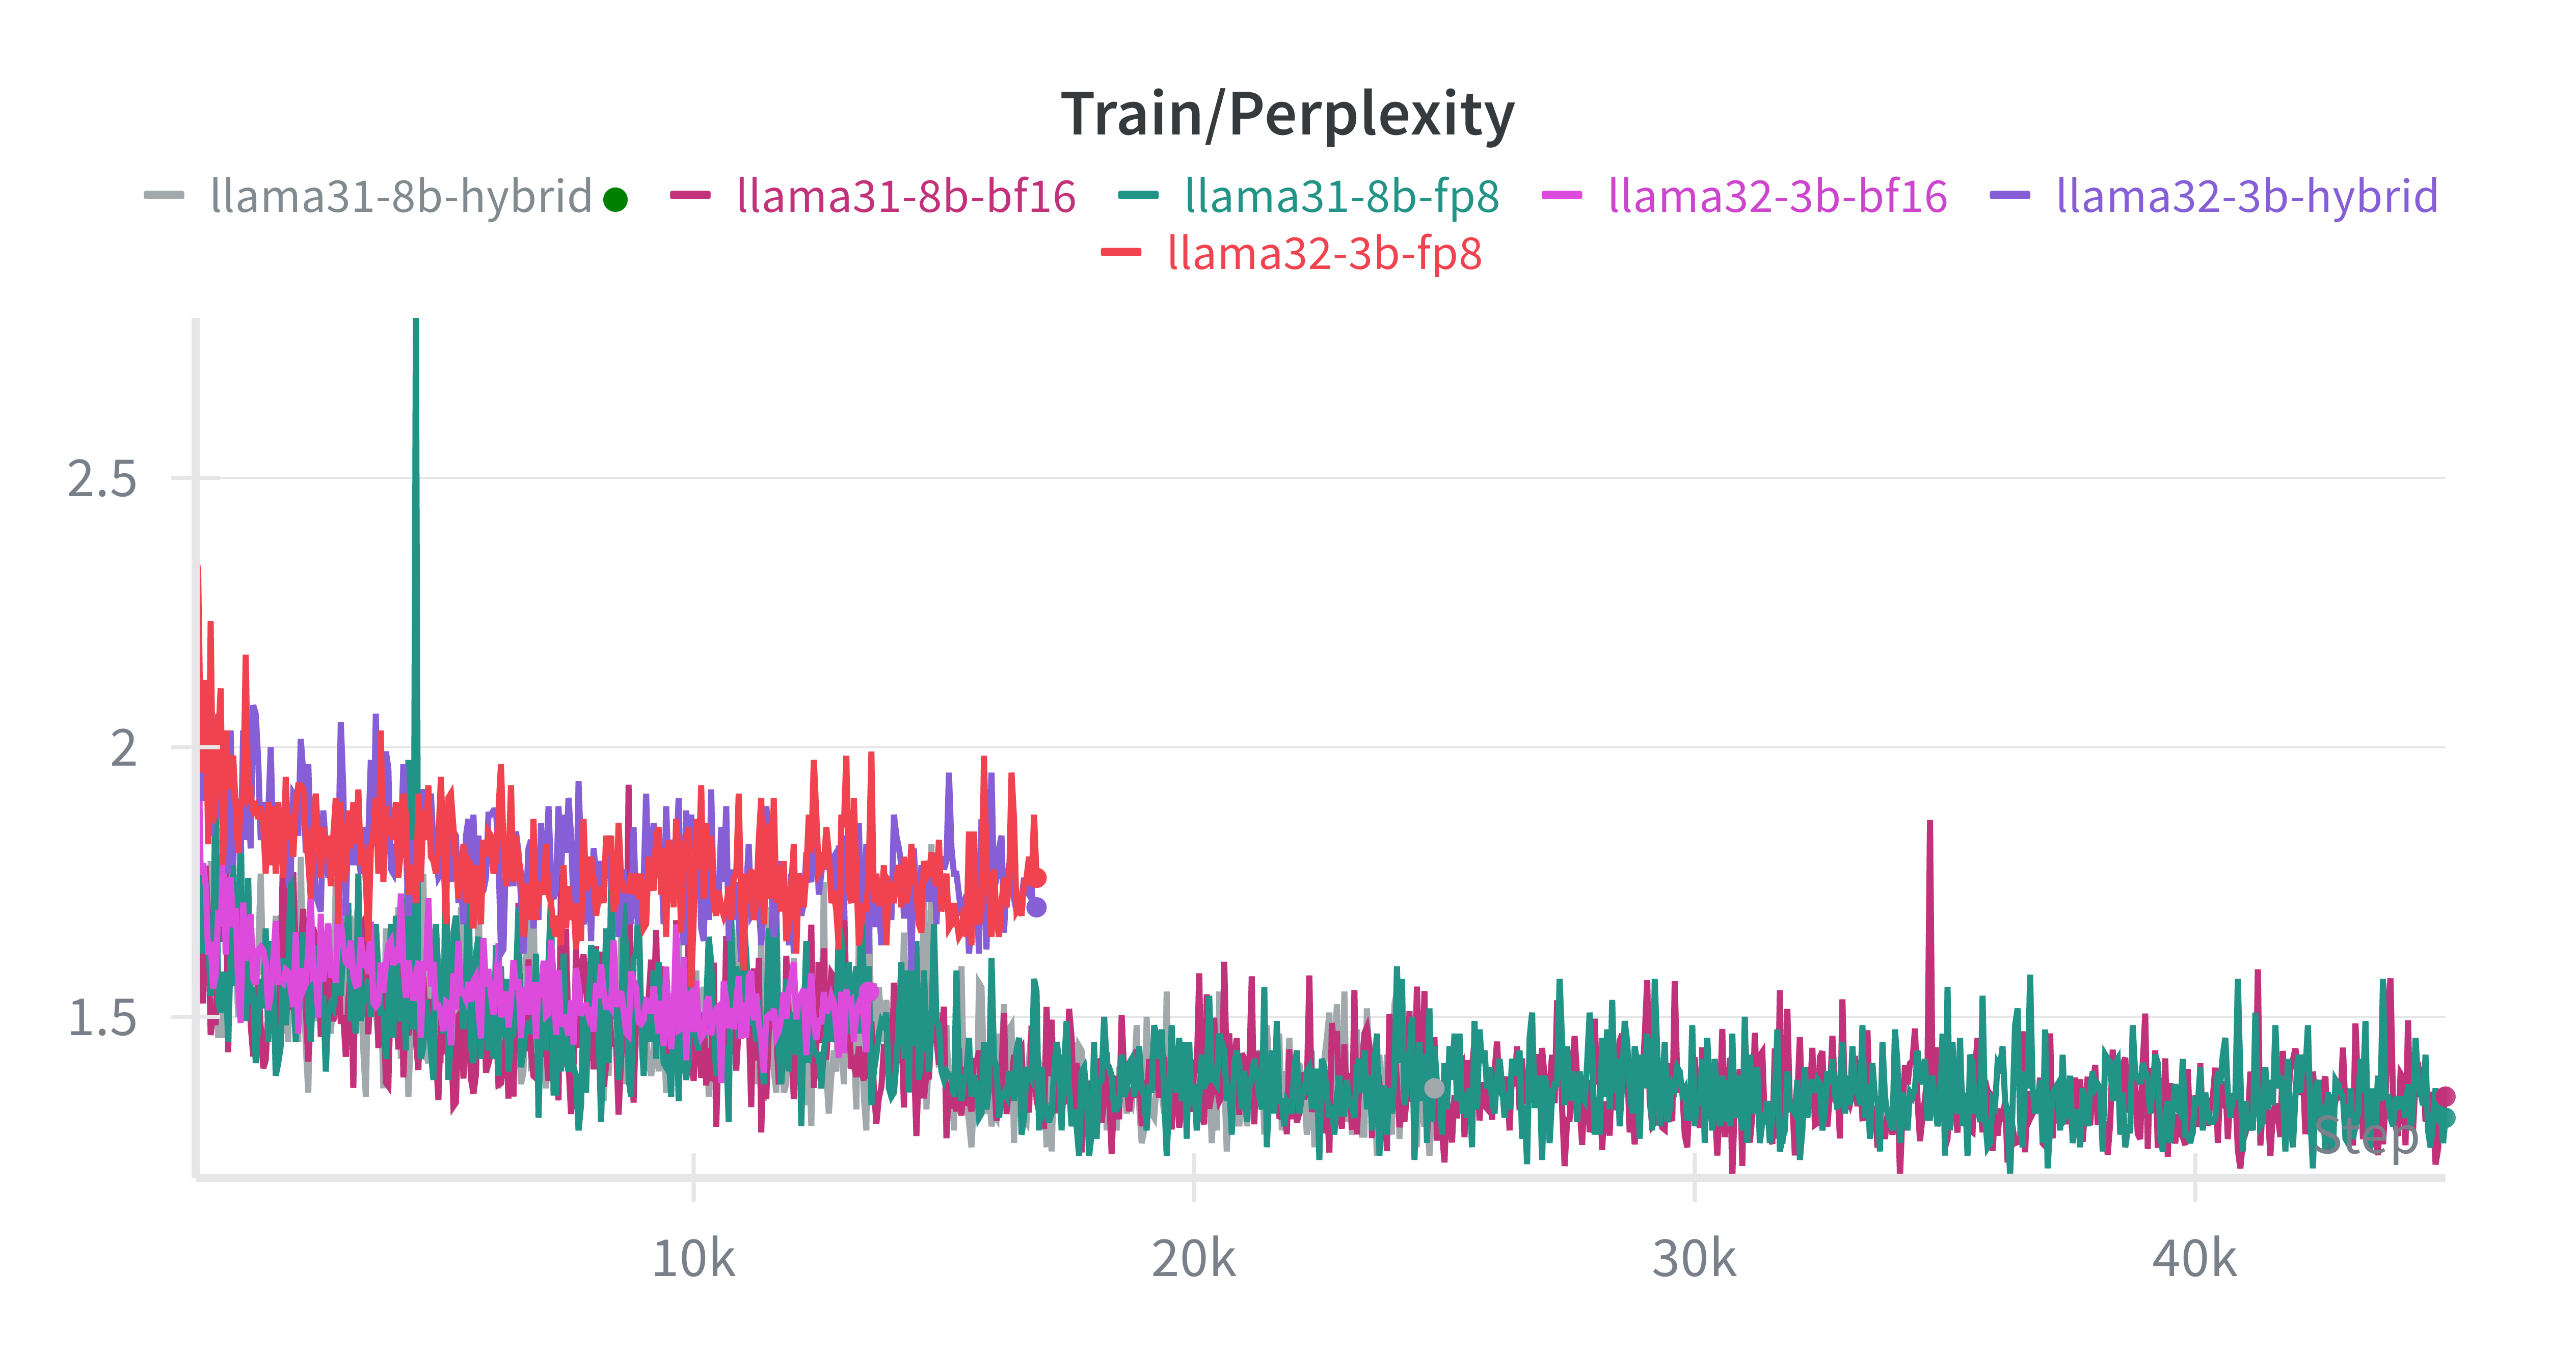
\includegraphics[width=\textwidth]{figures/train_perplexity.png}

    \vspace{0.3cm}

    \small
    \textbf{Observation:} Layer-wise FP8 maintains perplexity close to BF16, demonstrating effective precision-range trade-off.
\end{column}
\end{columns}

\end{frame}
